\documentclass[hyperref=colorlinks]{beamer}
\mode<presentation>
\usetheme{iclpt}
\setbeamertemplate{navigation symbols}{}
\setbeamertemplate{headline}{
\begin{beamercolorbox}[leftskip=.2cm,rightskip=.2cm,topskip=.2cm,ht=1.1cm,dp=0.1cm,wd=\textwidth]{institute in head/foot}
  
\includegraphics[height=1cm]{icl.pdf}
  \hfill
  
\includegraphics[height=1cm]{../Pics/CMS-Color.pdf}
\end{beamercolorbox}
}
\setbeamertemplate{footline}{
\begin{beamercolorbox}[ht=.55cm,dp=0.4cm,wd=\textwidth,leftskip=.3cm]{author in head/foot}%
  \begin{minipage}[c]{5cm}%
    \usebeamerfont{author in head/foot}
    \insertshortauthor 
    \insertshorttitle
    \end{minipage}\hfill%
  \insertframenumber{} / \pageref{lastframe}
  \hfill
  \begin{minipage}{6cm}
    \hfill
  \end{minipage}
\end{beamercolorbox}%
}

\usepackage{color}
\usepackage{tabularx,colortbl}
\usepackage{graphicx}
\usepackage{pdfpages}
\usepackage{feynmp}
\DeclareGraphicsRule{*}{mps}{*}{}

\title{\vspace{-0.2cm} New Framework Overview}
%\subtitle{Paper - HIG-13-030, PASs: HIG-13-013, HIG-13-018, HIG-13-028 \vspace{-0.7cm}}
\author[P. Dunne]{\underline{P. Dunne} }%\\ on behalf of the H$\rightarrow$invisible analysis groups} % A.M. Magnan and A. Nikitenko Joao Pela with \\ R. Aggleton, J. Brooke: Bristol \\ C.Asawangtrakuldee, Q.Li: Peking \\ P. Srimanobhas: Chulalongkorn \\ S. Kumar, K. Mazumdar: Mumbai}
\titlegraphic{
  \vspace{-0.7cm}
  %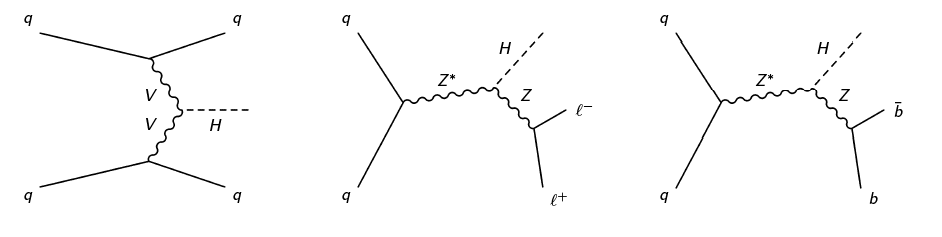
\includegraphics[width=\textwidth]{TalkPics/invcomb021213/feyndiags}
%% \begin{fmfgraph*}(100,70)
%%         \fmfleft{i1,i2}
%%         \fmfright{o1,o2,o3}
%%         \fmf{fermion}{i1,v1,o1}
%%         \fmf{fermion}{i2,v2,o3}
%%         \fmf{phantom,tension=4/5}{v1,v2}
%%         \fmffreeze
%%         \fmf{photon,label=$W,,Z$}{v1,v3}
%%         \fmf{photon,label=$W,,Z$}{v2,v3}
%%         \fmf{dashes}{v3,o2}
%%         \fmflabel{$q$}{i1}
%%         \fmflabel{$q$}{i2}
%%         \fmflabel{$q$}{o1}
%%         \fmflabel{$q$}{o3}
%%         \fmflabel{$H$}{o2}
%%       \end{fmfgraph*}
}
\date{}
\begin{document}
\begin{fmffile}{hig1330approvalfeynmandiags}

%TITLE PAGE
\section{Title}
\begin{frame}
  \titlepage
  
\end{frame}

%OUTLINE
\begin{frame}
  \frametitle{Overview}
  \begin{block}{}
    \scriptsize
    \begin{itemize}
    \item Summarise current framework
    \item Introduce new framework
    \item Compare W background estimates from both frameworks
    \item Twiki with instructions to have a go yourself can be found \href{https://twiki.cern.ch/twiki/bin/viewauth/CMS/VBFHinvisibleParkedData}{here}
    \end{itemize}
  \end{block}
\end{frame}

\begin{frame}
  \frametitle{Current framework}
  \begin{block}{}
    \scriptsize
    \begin{itemize}
    \item Current framework runs one batch job per sample
    \item[-] Job performs cuts, calculates weights and makes variations for systematics
    \item[-] Jobs take O(hours) to complete
    \item[-] With skimming on trigger this changes to O(minutes)
    \item Macros are then used to extract information from the output of these jobs and combine into results
    \item Changing cuts requires resending jobs
    \item Information about correlations between variables is hard to access
    \end{itemize}
  \end{block}
\end{frame}

\begin{frame}
  \frametitle{New framework}
  \begin{block}{}
    \scriptsize
    \begin{itemize}
    \item Use current framework to output a light ntuple
    \item Correlation information is kept in the light ntuple so it can be used for TMVA
    \item Use an analyser which runs modules over all the samples to produce results
    \item Light ntuples take O(minutes) to run over
    \end{itemize}
  \end{block}
\end{frame}

\begin{frame}
  \frametitle{Content of ntuples}
  \begin{block}{}
    \scriptsize
    \begin{itemize}
    \item Current FW ntuples contain full objects
    \item[-] Very flexible don't have to be rerun very often
    \item[-] Example can be found by following steps on \href{https://twiki.cern.ch/twiki/bin/viewauth/CMS/VBFHinvisibleParkedData}{twiki}
    \item New light ntuples just contain variables of interest for analysis and optimisation, without cuts
    \item[-] Can be remade in O(hours)
    \item[-] Current list of variables can be found in header file of light tree maker \href{https://github.com/ajgilbert/ICHiggsTauTau/blob/master/Analysis/HiggsNuNu/interface/LightTree.h}{here}
      \item[-] Will be changed as and when required
    \end{itemize}
  \end{block}
\end{frame}

\begin{frame}
  \frametitle{Checks of framework}
  \begin{columns}
    \column{1.1\textwidth}
  \begin{block}{}
    \scriptsize
    \begin{itemize}
    \item A module that performs the $W\rightarrow\mu/e\nu$ background estimates has been written
    \item Unweighted results are identical to old framework
    \item Weighted results are as below:
    \item[-] Note these numbers are different from those in our AN as they use the re-reco data
    \end{itemize}
    \begin{table}
      \begin{tabular}{|l||c|c||c|c|}
        \hline
        Result & Old FW munu & New FW munu & Old FW enu & New FW enu \\
        \hline
        NSMC & 123.0 & 121.9 & 124.2 & 122.3 \\
        NCMC & 371.0 & 370.0 & 113.4 & 116.0 \\
        NCData$-$NCBkg & 196.0 & 195.9 & 62.4 & 62.2 \\
        Result & 65.1 & 64.5 & 68.3 & 65.6 \\
        \hline
      \end{tabular}
    \end{table}
  \end{block}
  \end{columns}
\end{frame}

\begin{frame}
  \frametitle{Conclusions}
  \label{lastframe}

  \begin{block}{}
    \scriptsize
    \begin{itemize}
    \item New framework reproduces to couple of \% level results of old framework
    \item[-] difference from weighting, will investigate
    \item Instruction to try it out can be found \href{https://twiki.cern.ch/twiki/bin/viewauth/CMS/VBFHinvisibleParkedData}{here}
    \end{itemize}
  \end{block}

\end{frame}

\begin{frame}
  \frametitle{Backup}
\end{frame}


\end{fmffile}
\end{document}
